\chapter{Izpeljava gibanja sonde relativno na magnet ob nepravilni montaži}

Nepravilna montaža bo vplivala na obe Hallovi sondi simulacijskega modela enako. Vpliv izmika senzorja in magneta, na relativno gibnaje sonde nad magnetom bo prikazano na eni sondi. Na koncu poglavja je prikazan rezultat relativnega gibanja obeh sond simulacijskega modela na magnet.

Izmik sredine senzorja iz osi vrtenja bo med spreminjanjem dejanskega kota zasuka statičen, njegova lokacija se nebo spreminjala na os vrtenja. Ta izmik je poimenovan statična ekscentričnost.

Ob izmiku magneta iz osi vrtenja se pojavi opletanje magneta. Lokacija središča magneta se spreminja glede na določen zasuk magneta. Opletanje magneta je poimenovano dinamična ekscentričnost.

%V tem poglavju je  izpeljan vpliv napačne montaže , ki se pojavita zaradi neprimerne vgradnje. Napaki različno vplivati na izhodni podatek, zato se ju lahko obravna posamično. Preko analitične izpeljave je prikazano, kako se spreminja lokacija Hall-ove sonde glede na magnet ob pravilni montaži. Z vpeljavo dodatne ekscentričnosti v model se potek gibanja sonde glede na magnet spremeni. S poznavanjem lokacije sonde nad magnetom se lahko odčita pomerjena vrednost \Bz.

\section{Definicija koordinatnega sistema}

Kartezični koordinatni sistem, ima v izhodišču postavljen radialno polariziran magnet ($S_m(0, 0)$). V izhodišču se nahaja tudi os vrtenja ($S_r(0, 0)$). Na poljubno točko $H(x_0,y_0)$, vendar ne v izhodišče je postavljena Hall-ova sonda (slika \ref{fig:def_kks}).
\begin{figure}[h!]
	\centering
	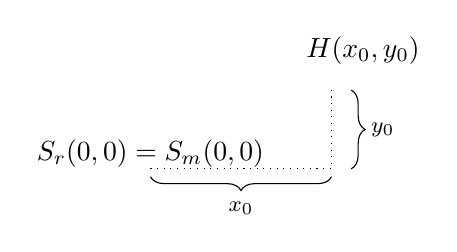
\begin{tikzpicture}

	\magnet {0} {0} {0}{ }{1};
	\hall {2.3}{1} {0};
	\draw [decorate,decoration={brace,amplitude=5pt,mirror},xshift= 0pt,yshift=0pt]
	(2.55,0) -- (2.55,1) node [black,midway,xshift= 0.4cm] 
	{\footnotesize $y_0$};
	\draw [decorate,decoration={brace,amplitude=5pt,mirror},xshift= 0pt,yshift=0pt]
	(0,-0.1) -- (2.3,-0.1) node [black,midway,yshift= -0.4cm] 
	{\footnotesize $x_0$};
	\draw[dotted](0,0)--(2.3,0)--(2.3,1) node[yshift = 0.5cm, xshift = 0.4 cm] {$H(x_0,y_0)$};
	\node at (0,0.2) {$S_r(0, 0)=S_m(0, 0)$};
	\end{tikzpicture}
	\caption{Definicija koordinatnega sistema z magnetom in Hall-ovo sondo}
	\label{fig:def_kks}
\end{figure}

Z zasukom magneta za kot $\theta$, se lokacija sonde glede na magnet spremeni. Nova lokacija sonde glede na magnet je enaka, če se namesto magnet, zavrti sondo za kot $-\theta$ . Nova lokacija sonde glede na magnet je v točki  $(x, y)$. Novo lokacijo sonde glede na magnet v odvisnosti od zasuka magneta za kot $\theta$, opiše enačba (\ref{equ:rotacija_hall}).

\begin{equation}
\label{equ:rotacija_hall}
\begin{bmatrix} x\\y \end{bmatrix}=
\begin{bmatrix} \cos(-\theta)&-\sin(-\theta)\\\sin(-\theta)&\cos(-\theta) \end{bmatrix}
\begin{bmatrix} x_0\\y_0 \end{bmatrix}
\end{equation}

Argument rotacijske matrike je $-\theta$. Z upoštevanjem lihosti funkcije sinus in sodosti funkcije kosinus\cite{Matematika1}, se (\ref{equ:rotacija_hall}) poenostavi v:
\begin{equation}
%\label{equ:rotacija_hall_simplify}
\begin{bmatrix} x\\y \end{bmatrix}=
\begin{bmatrix} \cos(\theta)&\sin(\theta)\\-\sin(\theta)&\cos(\theta) \end{bmatrix}
\begin{bmatrix} x_0\\y_0 \end{bmatrix}
\end{equation}

\begin{figure}[h!]
    \begin{subfigure}[b]{0.5\textwidth}
	\centering
		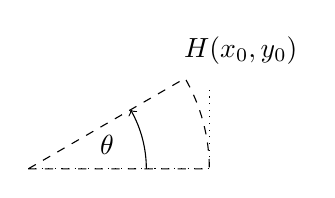
\begin{tikzpicture}
		[scale=1, every node/.style={scale=1}]
				\magnet {0} {0} {30}{}{1}
				\hall {2.3}{0+1} {0};
				\draw[dotted](0,0)--(2.3,0)--(2.3,1) node[yshift = 0.5cm, xshift = 0.4 cm] {$H(x_0,y_0)$};
				\draw [dashed](0,0)--(2.3,0) arc (0:30:2.3)--(0,0);
				\node at(1,0.3){$\theta$};
                \draw [->] (1.5,0) arc (0:30:1.5);
		\end{tikzpicture}
	\caption{Zasukan magnet za kot $\mathrm{\theta}$}
	\label{subfig:zasuk_magnet}
\end{subfigure}
\begin{subfigure}[b]{0.5\textwidth}
	\centering
		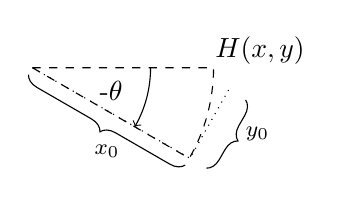
\begin{tikzpicture}[scale=1, every node/.style={scale=1}]		
				\magnet {0} {0} {0}{}{1}
				\hall {2.4919}{-0.2839} {-30};
				\draw [dashed](0,0)--(2.3,0) arc (0:-30:2.3)--(0,0);
				\node at(1,-0.3){-$\theta$};
                \draw [->] (1.5,0) arc (0:-30:1.5);
                
                \draw[dotted](0,0)--(2,-1.15)--(2.49,-0.2839) node[yshift = 0.5cm, xshift = 0.4cm] {$H(x,y)$};
                \draw [decorate,decoration={brace,amplitude=5pt,mirror},xshift= 0pt,yshift=0pt]
                (2.2084,-1.275) -- (2.7084,-0.40897) node [black,midway,xshift= 0.4cm] 
                {\footnotesize $y_0$};
                \draw [decorate,decoration={brace,amplitude=5pt,mirror},xshift= 0pt,yshift=0pt]
                (-0.05,-0.086603) -- (1.9419,-1.2366) node [black,midway,yshift= -0.4cm] 
                {\footnotesize $x_0$}; 
		\end{tikzpicture}
	
	\caption{Zasukan senzor za kot $\mathrm{-\theta}$}
	\label{subfig:zasuk_hall}
\end{subfigure}

\caption{Sprememba položaja glede na magnet ob rotaciji}
\label{fig:zasuk_magneta}

\end{figure}



\section{Izpeljava gibanja lokacije Hallove sonde na magnet pri dinamični ekscentričnosti}

Magnet je postavljen v izhodišce koordinatnega sistema $S_m(0,0)$, kjer je tudi os vrtenja $S_r(0,0)$. Dinamična ekscentričnost povzroči premik središča magneta v točko $S_{m1}(\Delta x_d,\Delta y_d)$ (Slika \ref{fig:def_din_eks}). Os vrtenja je ostaja v izhodišču koordinatnega sistema. Središce magneta $S_{m1}(\Delta x_d,\Delta y_d)$ ob rotaciji opiše okoli osi vrtenja krožnico z radijem $\sqrt{\Delta x_d^2+\Delta y_d^2}$.% (\ref{equ:rotacija_hall_din_sonda}).

\begin{figure}[h!]
	\centering
	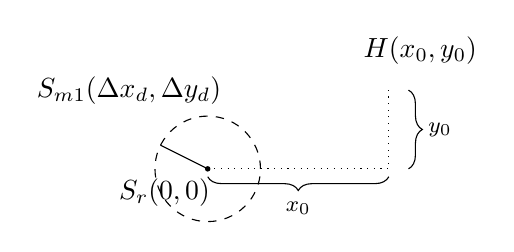
\begin{tikzpicture}
		\magnet {-0.6} {0.3} {0}{ }{1};
		\hall {2.3}{1} {0};
		\kks{3}
		\draw [dashed]  (0,0) circle (0.67);
		\draw (0,0)--(-0.6,0.3);
		\fill (0,0) circle [radius=1pt];
		\node at (-0.55,-0.3){$S_r(0,0)$};
		\node at(-1,1){$S_{m1}(\Delta x_d,\Delta y_d)$};
		\draw [decorate,decoration={brace,amplitude=5pt,mirror},xshift= 0pt,yshift=0pt]
		(2.55,0) -- (2.55,1) node [black,midway,xshift= 0.4cm] 
		{\footnotesize $y_0$};
		\draw [decorate,decoration={brace,amplitude=5pt,mirror},xshift= 0pt,yshift=0pt]
		(0,-0.1) -- (2.3,-0.1) node [black,midway,yshift= -0.4cm] 
		{\footnotesize $x_0$};
		\draw[dotted](0,0)--(2.3,0)--(2.3,1) node[yshift = 0.5cm, xshift = 0.4 cm] {$H(x_0,y_0)$};
	\end{tikzpicture}
	\caption{Definicije dinamične ekscentričnosti}
	\label{fig:def_din_eks}
\end{figure}

%\begin{equation}
%\label{equ:rotacija_hall_din_sonda}
%\begin{bmatrix} \cos(\theta)&\sin(\theta)\\-\sin(\theta)&\cos(\theta) \end{bmatrix}\cdot
%\begin{bmatrix} x_d\\y_d \end{bmatrix}
%\end{equation}
%S (\ref{equ:rotacija_hall_din_sonda}) je izraženo gibanje središče magneta na Hallovo sondo. Celoten sistem se vrti okoli osi vrtenja $S_r(0,0)$. Ob zasuku magneta se spreminja razdalja med sondo in središčem magneta po (\ref{equ:razdaljamagnetsonda}).
%\begin{equation}
%\label{equ:razdaljamagnetsonda}
%\begin{bmatrix} x_0\\y_0 \end{bmatrix}-
%\begin{bmatrix} \cos(\theta)&\sin(\theta)\\-\sin(\theta)&\cos(\theta) \end{bmatrix}\cdot
%\begin{bmatrix} x_d\\y_d \end{bmatrix}
%\end{equation}
%Enako kot v prejšnjem poglavju se sedaj sondo zasuka v nasprotno 
%\begin{equation}
%\label{equ:rotacija_hall_din_1}
%\begin{bmatrix} x\\y \end{bmatrix}=
%\begin{bmatrix} \cos(\theta)&-\sin(\theta)\\ \sin(\theta)&\cos(\theta) \end{bmatrix}
%\cdot \begin{pmatrix}
%\begin{bmatrix} x_0\\y_0 \end{bmatrix}-
%\begin{bmatrix} \cos(\theta)&\sin(\theta)\\-\sin(\theta)&\cos(\theta) \end{bmatrix}\cdot
%\begin{bmatrix} x_d\\y_d \end{bmatrix}\end{pmatrix}
%\end{equation}
%
%(\ref{equ:rotacija_hall_din_1}) se poenostavi:
%\begin{equation}
%\label{equ:rotacija_hall_din}
%\begin{bmatrix} x\\y \end{bmatrix}=
%\begin{bmatrix} \cos(\theta)&\sin(\theta)\\-\sin(\theta)&\cos(\theta) \end{bmatrix}
%\begin{bmatrix} x_0\\y_0 \end{bmatrix}
%-
%\begin{bmatrix} \Delta x_d\\\Delta y_d \end{bmatrix}
%\end{equation}
Naj ostane magnet v izhodišču $S_m(0,0)$ in naj se spremeni lokacija Hallove sonde in os vrtnja za $(-\Delta x_d,-\Delta y_d)$ (Slika \ref{fig:def_din_eksbac}). Sondo se tako kot v prejšnjem poglavju zavrti v nasprotno stran okoli osi vrtenja. Os vrtenja je v točki $(-\Delta x_d,-\Delta y_d)$. Sonda se giblje po krožnici s središčem v točki $(-\Delta x_d,-\Delta y_d)$. Spreminjanje lokacije sonde glede na magnet opiše (\ref{equ:rotacija_hall_din})
\begin{equation}
\label{equ:rotacija_hall_din}
\begin{bmatrix} x\\y \end{bmatrix}=
\begin{bmatrix} \cos(\theta)&\sin(\theta)\\-\sin(\theta)&\cos(\theta) \end{bmatrix}
\begin{bmatrix} x_0\\y_0 \end{bmatrix}
-
\begin{bmatrix} \Delta x_d\\\Delta y_d \end{bmatrix}
\end{equation}

\begin{figure}[h!]
	\centering
	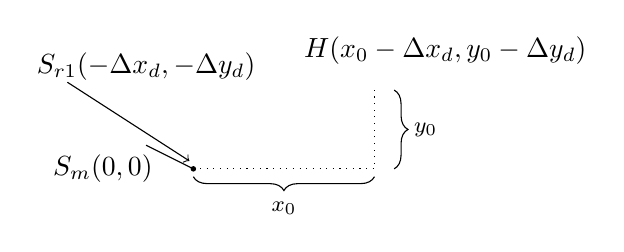
\begin{tikzpicture}
	\magnet {0} {0} {0}{ }{1};
	\hall {2.3+0.6}{1-0.3} {0};
	\kks{3}
	\draw (0,0)--(0.6,-0.3);
	\fill (0.6, -0.3) circle [radius=1pt];
	\node at (-0.55,-0.3){$S_m(0,0)$};
	\node at(0,1){$S_{r1}(-\Delta x_d,-\Delta y_d)$};
	\draw [->](-1,0.8)--(0.55,-0.2);
	\draw [decorate,decoration={brace,amplitude=5pt,mirror},xshift= 0pt,yshift=0pt]
	(2.55+0.6,0-0.3) -- (2.55+.6,1-.3) node [black,midway,xshift= 0.4cm] 
	{\footnotesize $y_0$};
	\draw [decorate,decoration={brace,amplitude=5pt,mirror},xshift= 0pt,yshift=0pt]
	(0+.6,-0.1-.3) -- (2.3+.6,-0.1-.3) node [black,midway,yshift= -0.4cm] 
	{\footnotesize $x_0$};
	\draw[dotted](0+.6,0-.3)--(2.3+.6,0-.3)--(2.3+.6,1-.3) node[yshift = 0.5cm, xshift = 0.9 cm] {$H(x_0-\Delta x_d,y_0-\Delta y_d)$};
	\end{tikzpicture}
	\caption{Premik osi vrtenja in sonde za velikost dinamične ekscentričnosti}
	\label{fig:def_din_eksbac}
\end{figure}

%
%\begin{figure}[h!]
%	\centering
%	\begin{tikzpicture}
%		\magnet {0} {0} {0}{$S_{m}(0,0)$}{1};
%		\draw (0,0)--(-0.6,-0.3);
%		\fill (-0.6,-0.3) circle [radius=1pt];
%		\node at (0,-0.6){$S_0(-\Delta x_d,-\Delta y_d)$};
%		\hall {1.7}{-0.3} {0};
%		\kks{3}
%	\end{tikzpicture}
%	\caption{Shema definicije dinamične ekscentričnosti vpliva na Hall-ovo sondo}
%	\label{fig:def_din_eks_na_stator}
%\end{figure}
%
%Sistema prikazana na slikah \ref{fig:def_din_eks} in \ref{fig:def_din_eks_na_stator}, se v začetnih legah ne razlikujeta. Sedaj zarotirajmo Hall-ovo sondo okoli osi vrtenja $S_0(-\Delta x_d,-\Delta y_d)$. Hall-ova sonda se giblje glede na magnet enako, kot če bi magnet zavrteli z dinamično ekscentričnostjo (Slika \ref{fig:def_din_eks}). Gibanje Hall-ove sonde na magnet je izraženo kot gibanje po krožnici s središčem v točki $(-\Delta x_d,-\Delta y_d)$.
%
%\begin{figure}[h!]
%	\centering
%	\begin{tikzpicture}
%		\magnet {0} {0} {0}{}{1};
%		\draw [dotted]  (-0.6,-0.3) circle (2.3);
%		\draw (0,0)--(-0.6,-0.3);
%		\fill (-0.6,-0.3) circle [radius=1pt];
%		\hall {1.39}{-1.45} {-30};
%		\draw [dashed](-0.6,-0.3)--(1.7,-0.3) arc(0:-30:2.3)--(-0.6,-0.3);
%		\node at(0.4,-0.6){$-\theta$};
%        \draw [->] (0.9,-0.3) arc (0:-30:1.5);
%		\kks{3}
%	\end{tikzpicture}
%	\caption{Potek Hall-ove sonde ob rotaciji glede na magnet ob dinamični ekscentričnosti}
%	\label{fig:potek_sonde_din_eks}
%\end{figure}
%
%Potek Hall-ove sonde ob rotaciji z upoštevanjem dinamične ekscentričnosti lahko zapišemo kot rotacijo z dodatno enosmerno komponento(\ref{equ:rotacija_hall_simplify}).
%
%
%
%V (\ref{equ:rotacija_hall_din}) lahko izrazimo - in izraz se poenostavi.
%
%\begin{equation}
%\label{equ:rotacija_hall_din_simplify}
%\begin{bmatrix} x\\y \end{bmatrix}=
%\begin{bmatrix} \cos(\theta)&-\sin(\theta)\\\sin(\theta)&\cos(\theta) \end{bmatrix}
%\begin{bmatrix} x_0\\y_0 \end{bmatrix}
%-
%\begin{bmatrix} \Delta x_d\\\Delta y_d \end{bmatrix}
%\end{equation}

\section{Izpeljava gibanja lokacije Hall-ove sonde na magnet pri statični ekscentričnosti}

Statična ekscentričnost se pojavi, ob izmiku Hallove sonde iz njene osnovne lege v  $H_1(x_0+\Delta x_s, y_0+\Delta y_s)$. Z zasukom magneta je razdalja med sondo in osjo vrtenja konstantna. Z miselnim obratom vrtenja sonde v nasprotni smeri se gibanje sonde izrazi kot gibanje po krožnici z novim radijem $\sqrt{(x_0+\Delta x_s)^2+(y_0+\Delta y_s)^2}$ (\ref{equ:rotacija_hall_stat}).


\begin{figure}[h!]
	\centering
	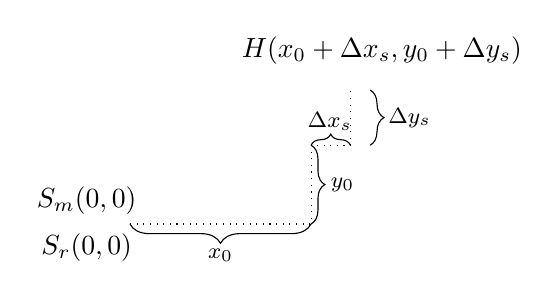
\begin{tikzpicture}
	\kks{3}
	\magnet {0} {0} {0}{}{1};
	\hall {2.3+0.5}{1+0.7} {0};

	\node at (-0.55,-0.3){$S_r(0,0)$};
	\node at(-0.55,0.3){$S_{m}(0,0)$};
	\draw [decorate,decoration={brace,amplitude=5pt,mirror},xshift= 0pt,yshift=0pt]
	(2.3,0) -- (2.3,1) node [black,midway,xshift= 0.4cm] 
	{\footnotesize $y_0$};

	\draw [decorate,decoration={brace,amplitude=7pt,mirror},xshift= 0pt,yshift=0pt]
	(0,0) -- (2.3,0) node [black,midway,yshift= -0.4cm] 
	{\footnotesize $x_0$};
	\draw[dotted](0,0)--(2.3,0)--(2.3,1)--(2.8,1)--(2.8,1.7) node[yshift = 0.5cm, xshift = 0.4 cm] {$H(x_0 + \Delta x_s ,y_0+ \Delta y_s)$};
	
	\draw [decorate,decoration={brace,amplitude=4pt},xshift= 0pt,yshift=0pt]
	(2.3,1) -- (2.8,1) node [black,midway,xshift = -0.4 ,yshift= 0.3cm] 
	{\footnotesize $\Delta x_s$};
	
	\draw [decorate,decoration={brace,amplitude=5pt,mirror},xshift= 0pt,yshift=0pt]
	(3.05,1)--(3.05,1.7) node [black,midway,xshift= 0.5cm] 
	{\footnotesize $\Delta y_s$};
%	\draw[<->,dotted] (0,0)--(0,-0.6);
%	\draw[<->,dotted] (0, -0.6)--(0.6,-0.6);
%	\draw[dotted] (2.9,-0.6)--(0.6,-0.6);
%	\node at (0.4,-0.3){$\Delta y_s$};
%	\node at (0.4,-0.8){$\Delta x_s$};
	\end{tikzpicture}
	\caption{Definicije statične ekscentričnosti}
	\label{fig:def_sta_eks}
\end{figure}
%Po enakem razmišljanju kot v zgornjih poglavjih, sedaj zarotirajmo Hall-ovo sondo za kot \kol{-\theta} okoli izhodišča. Hall-ova sonda se giblje po krožnici z radijem $\sqrt{(x_0+\Delta x_s)^2+(y_0+\Delta y_s)^2}$.
%Statična ekscentričnost tako vpliva le na spremembo radija krožnice, ki jo opiše Hall-ova sonda ob rotaciji nad magnetom.
%\begin{figure}[h!]
%	\centering
%	\begin{tikzpicture}
%	\magnet {0} {0} {0}{}{1};
%	\hall {1.69}{-1.67} {-30};
%	\draw[<->,dotted] (0,0)--(-0.3,-0.52);
%	\draw[dotted] (1.69,-1.67)--(-0.3,-0.52);
%	\draw [dashed] (0,0) -- (2.377,0) arc(0:-30:2.377)--(0,0);
%	\node at (0.8,-0.2) {\kol{-\theta}};
%	\draw [dotted] (0,0)circle[radius=2.377];
%%    \draw [dotted, <->] (0,0)--(2.06,1.19);
%%    \node at (4.03,0.6){$\sqrt{(x_0+\Delta x_s)^2+(y_0+\Delta y_s)^2}$};
%	\draw [dotted, <->] (0,0)--(1.69,-1.67);
%    \draw [->] (1.5,0) arc (0:-30:1.5);
%	\end{tikzpicture}
%	\caption{Potek sonde ob vrtenju glede na magnet ob statični ekscentričnosti}
%	\label{fig:def_sta_eks_stat}
%\end{figure}
Novo lokacijo sonde glede na magnet opiše (\ref{equ:rotacija_hall_stat}). Ob povzročeni statični ekscentričnosti se sonda giblje po drugem radiju.
\begin{equation}
\label{equ:rotacija_hall_stat}
\begin{bmatrix} x\\y \end{bmatrix}=
\begin{bmatrix} \cos(\theta)&\sin(\theta)\\-\sin(\theta)&\cos(\theta) \end{bmatrix}
\begin{bmatrix} x_0+\Delta x_s\\y_0+\Delta y_s \end{bmatrix}
\end{equation}







\section{Končna enačba za določanje lokacije Hall-ove sonde}

%Do sedaj smo postopoma izpeljali enačbe za:
%\begin{itemize}
%  \item sistem magneta in Hall-ove sonde ob pravilni montaži
%  \item sistem magneta in Hall-ove sonde z dinamično ekscentričnostjo magneta
%  \item sistem magneta in Hall-ove sonde s statično ekscentričnostjo Hall-ove sonde
%\end{itemize}

(\ref{equ:rotacija_hall_din}) in (\ref{equ:rotacija_hall_stat}) sta med seboj neodvisni zato se ju lahko združi. 
Z miselnim obratom rotacije sonde v nasprotno smer, kot bi se drugače vrtel magnet, so bili pridobljeni rezultati lokacije sonde relativno na magnet.
Dinamična ekscentričnost vpliva na premik krožnice, po kateri se navidezno giblje sonda. Statična ekscentričnost, povzroči spremembo radija, po kateri se navidezno giblje sonda.

\begin{equation}
\label{equ:rotacija_hall_koncna}
\begin{bmatrix} x\\y \end{bmatrix}=
\begin{bmatrix} \cos(\theta)&\sin(\theta)\\-\sin(\theta)&\cos(\theta) \end{bmatrix}
\begin{bmatrix} x_0+\Delta x_s\\y_0+\Delta y_s \end{bmatrix}-
\begin{bmatrix} \Delta x_d\\\Delta y_d \end{bmatrix}
\end{equation}






%Ogledali smo si, kako je ob rotaciji locirana Hall-ova sonda glede na magnet. Ogledali smo si tudi, kako na lokacijo sonde vplivati dinamična in statična ekscentričnost. S poznavanjem magnetnega polje $B_z=B_z(x , y)$, lahko določimo kakšno vrendost polja $B_z$ pomeri Hall-ova sonda ob rotaciji ($B_z=B_z(\theta)$). Ob poznavanju polja $B_z$, lahko določimo zasuk magneta glede na postavitev Hallove sonde.


%\chapter{Izpeljava poteka polja $B_z(\theta)$ in ocena napake zaradi ekscentričnosti}
%
%%V tem poglavju si bomo ogledali kakšno magnetno polje  pomeri Hall-ova sonda. Ogledali si bomo magnet, ter kako senzor RM44 meri magnetno polje. Preko pomirjenega polja, bomo izračunali kakšna je napake pomerjenega kota od referenčnega in kako se napaka spreminja z ekscentričnostjo.
%
%\section{Definicija  gostote magnetnega polja $B_z$}
%
%Predlagan magnet s strani proizvajalca senzorja je radialno magnetiziran s premerom 4 mm in višino 4 mm (slika \ref{magnet4mm}).
%\begin{figure}[h]
%	\centering
%	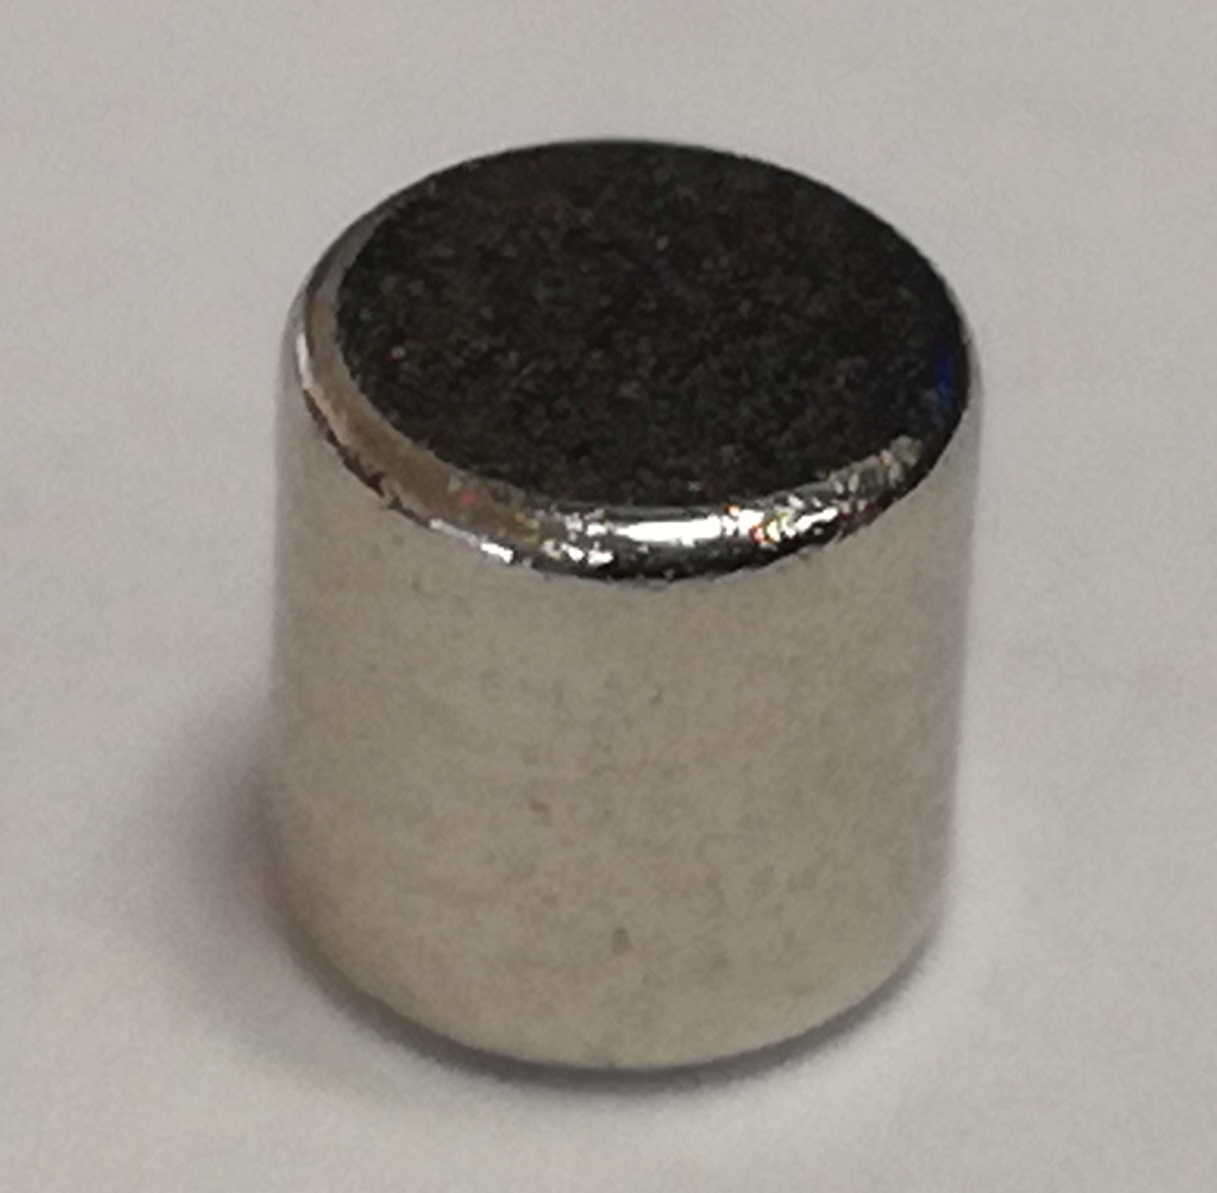
\includegraphics[width=0.75\columnwidth]{./Slike/magnet4mm.png}
%	\caption{Primer magneta predlagan s strani proizvajalca RLS}
%	\label{magnet4mm}
%\end{figure}
%Dajalnik pozicije RM44 meri z-komponento gostote magnetnega polja \cite{AM8192}. Potek komponente $B_z$ nad cilindričnim magnetom je prikazan na sliki \ref{fig:magnetno_polje}.
%
%%Magsnetno polje  v prostoru lahko izračunamo z Biot-Savartovim zakonom. Poznati moramo specifikacije trajnega magneta in izračunati integral po prostoru. Tako dobimo v poljubni točki v prostoru vrednost B.  Hall-ove sonde v senzorju RM44 merijo le z-komponento magnetnega polja, zato se lahko osredotočimo le nanjo. Odvistnost z-komponente vektorja B na konstantni višini od magneta je vidno na sliki \ref{fig:magnetno_polje}.
%
%
%
%\begin{figure}[h]
%	\centering
%		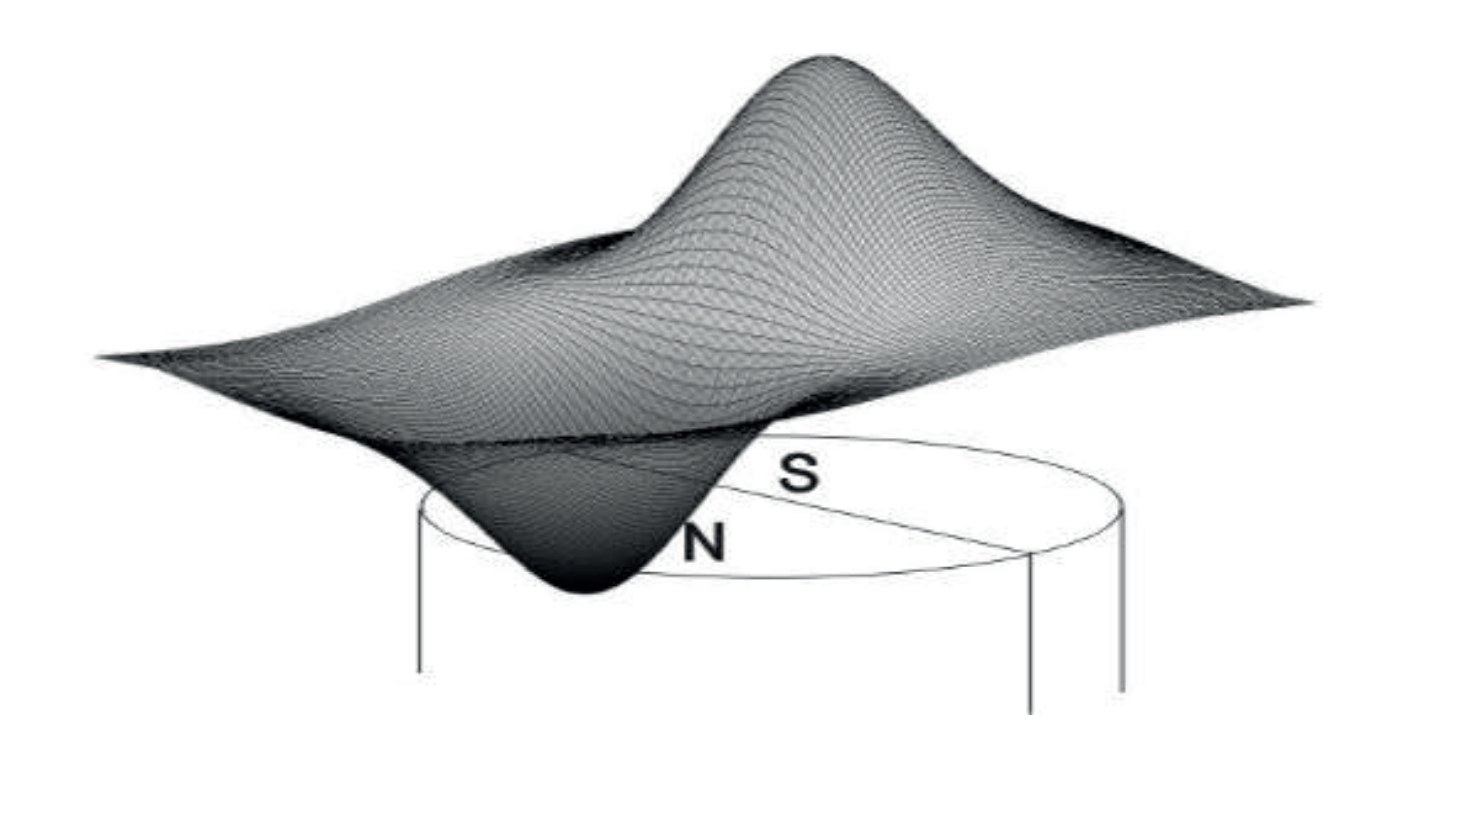
\includegraphics[width=0.75\columnwidth]{./Slike/magnetno_polje.jpg}
%	\caption{z-komponenta vektorja gostote magnetnega polja nad cilindričnim magnetom \cite{AM8192}}
%	\label{fig:magnetno_polje}
%\end{figure}
%
%
%Potek z-komponente se lahko izračuna po Biot-Savartovim zakonom oz. z numerično seštevanjem prispevke posameznih delčkov magneta. Za oceno napake, se magnetno polje z komponente v okolici osi vrtenja magneta aproksimira z ravnino (\ref{equ:poljeB}).
%
%\begin{equation}
%\label{equ:poljeB1}
%B_z(x,y)=k\cdot x.
%\end{equation}
%
%Aproksimacija zadostuje za oceno napake. S poznavanjem lokacije sonde glede na magnet, se lahko izračuna merjena komponenta magnetnega polja. Aprokisimirano polje je linearno odvisno od x komponente (\ref{equ:poljeB}). Za lažje razumevanje naj bo $k$ enak 1.
%
%\section{Postavitev Hallovih sond in pomerjeno polje v odvistnosti od ekscentričnosti}
%%Sedaj si oglejmo, kako bi določili kot zasuka poljubne točke okoli izhodišča. Definirajmo kartezični koordinatni sistem, in v njem poljubno točko $(x_0,y_0)$, ki ni v izhodišču(Slika \ref{fig:dolocitev_kota}).
%%Za določanje kota $\varphi$ je potrebno poznati poznati položaj točke. Kot $\varphi$ določimo preko trigonometrične funkcije $\arctan$: $$\varphi=\arctan\frac{y_0}{x_0}$$
%%
%%
%%
%%\begin{figure}[h!]
%%	\centering
%%	\begin{tikzpicture}[scale=4]
%%	\CaCS{0.75}{0}{0}
%%	\draw [->,thick](0,0)--(-0.5,0.2855);
%%	\draw (0.15,0) arc (0:150:0.15);
%%	\node at (0.05,0.05){$\varphi$};
%%%	\node at (-0.5,0.285) {\textbullet};
%%	\node at (-0.32,0.35) {($x_0$,$y_0$)};
%%	\end{tikzpicture}
%%	\caption{Slika za pomoč pri določanju kota}
%%	\label{fig:dolocitev_kota}
%%\end{figure}
%%
%%
%%Za določitev kota $\varphi$  je dovolj poznati že projekciji vektorja na koordinatni osi(slika \ref{fig:dolocitev_kota_2}),
%%
%%\begin{figure}[h!]
%%	\centering
%%	\begin{tikzpicture}[scale=4]
%%	\CaCS{0.75}{0}{0}
%%	\draw [->,thick](0,0)--(-0.5,0.2855);
%%	\draw (0.15,0) arc (0:150:0.15);
%%	\node at (0.05,0.05){$\varphi$};
%%	\draw [dashed] (-0.5,0.2855)--(-0.5,0);
%%	\draw [dashed] (-0.5,0.2855)--(0,0.2855);
%%	%	\node at (-0.5,0.285) {\textbullet};
%%%	\node at (-0.32,0.35) {($x_0$,$y_0$)};
%%	\node at(-0.5,-0.1){$x_0$} ;
%%	\node at(0.1,0.2855){$y_0$};
%%	\end{tikzpicture}
%%	\caption{Slika za pomoč pri določanju kota}
%%	\label{fig:dolocitev_kota_2}
%%\end{figure}
%%
%%
%%če poznamo projekciji točke na koordinatni osi, je to zadosten pogoj za določitev kota $\varphi$.
%%Projekcijo lahko pridobimo če opazujemo projekciji položaja točke v koordinatnih oseh.
%%
%%Sedaj si predstavljajmo da ta poljubna točka predstavlja enega od polov magneta. Za poznavanje zasuka pola magneta, je dovolj odčitanje polja na koordinatnih oseh. Hall-ovi sondi ne smeti biti postavljeni na isto koordinatno os. Ni nujno da sta sondi postavljeni pravokotno druga na drugo, si pa s tem prihranimo korak v katerem bi bilo potrebno izračunati projekcijo na pravokotni koordinatni osi.
%%
%%Iz zgornjega razmisleka lahko sedaj smiselno postavimo Hall-ovi sondi v koordinatni sistem. Najprimerneje ju je postaviti na koordinatni osi (Slika \ref{fig:zacetna_postavitev_sond}). Sondi postavimo na enako razdaljo od izhodišča $r_0$. Tako bo zajem poteka polja ob rotaciji magneta enak, le fazno zamaknjeno.
%
%
%Za izračun kota je potrebno poznati polje v vsaj dveh točkah nad magnetom. Simulacijski model vsebuje 2 Hallovi sondi na koordinatnih oseh, oddaljeni od izhodišča za $r_0$.
%
%\begin{figure}[h!]
%	\centering
%	\begin{tikzpicture}[scale=1]
%	\CaCS{3}{0}{0}
%	\senzorja{0}{0}{0}
%%	\magnet {0} {0} {10}{ }{0}
%	\node at (2.0,-0.5){$\mathrm{H}_1(r_0,0)$};
%	\node at (-1,2.3){$\mathrm{H}_2(0, r_0)$};
%	\end{tikzpicture}
%	\caption{Začetna postavitev Hallovih sond}
%	\label{fig:zacetna_postavitev_sond}
%\end{figure}
%
%S poznavanjem položaja sonde glede na magnet (\ref{equ:rotacija_hall_koncna}) in funkcije polja (\ref{equ:poljeB}) se lahko določi potek polja sonde. Sondi ob obratu vsaka pomeri svoje polje. Potek polja pomerjen s sondo v abcisni osi ($H_1$), je v idealni montaži podoben signalu kosinus, zato je poimenovan $B_{cos}$. Potek polja pomerjenega s sondo v ordinatni osi ($H_2$) je za $90^\circ$ zamaknjeno proti $B_{cos}$, zato je potek imenovan $B_{sin}$.
%
%\begin{equation}\label{equ:Bx_splosna}
%cos=B_{H_1}(\theta,r_0,\Delta x_s, \Delta y_s, \Delta x_d)= r_0 \cos\theta +\Delta x_s \cos\theta +\Delta y_s \sin\theta -\Delta x_d
%\end{equation}
%\begin{equation}\label{equ:By_splosna}
%sin=B_{H_2}(\theta,r_0,\Delta x_s, \Delta y_s, \Delta x_d)= r_0 \sin\theta +\Delta x_s \cos\theta +\Delta y_s \sin\theta-\Delta x_d
%\end{equation}
%
%%Zajeta signala bom od tu naprej imenoval sinus ($B_{sin}$) in cosinu ($B_{cos}$), ker je to njuna osnovna oblika.
%\subsection{Sprememba magnetnega polja zaradi ekscentričnosti}
%
%%Oglejmo si primer kakšno polje zajameti Hall-ovi sondi, ko ekscentričnosti ni. $B_{sin}$ in $B_{cos}$ izraza se poenostavita in dobimo poteka v obliki sinusa ter kosinusa z enako amplitudo (Slika \ref{./Napake/sincos_00}).
%
%%\slikaeps{Poteka $B_{sin}$ in $B_{cos}$ brez ekscentričnosti pri $r_0 = 1$ mm}{./Napake/sincos_00}
%%\newpage
%%Upoštevajmo sedaj le statični ekscentričnosti $\Delta x_s$ in $\Delta y_s$. $\Delta x_d$ postavimo na 0.   Enačbi (\ref{equ:Bx_splosna}) in (\ref{equ:By_splosna}) lahko preuredimo v izraza:
%
%Iz izrazov (\ref{equ:Bx_splosna}) in (\ref{equ:Bx_splosna}) brez upoštevanja ekscentričnosti sta $B_{sin}$ in $B_{cos}$ enake amplitude ter fazno zamaknjena za $90^\circ$. Z upoštevanjem statične ekscentričnosti se med $B_{sin}$ in $B_{cos}$ zmanjša fazni kot ter spremni amplituda (\ref{equ:Bx_stat}) (\ref{equ:By_stat}). Ob dinamični ekscentričnosti signala pridobita enosmerni komponenti (\ref{equ:Bx_din}) (\ref{equ:By_din}).
%
%
%\begin{equation}
%\label{equ:Bx_stat}
%cos(\theta,r_0,\Delta x_s, \Delta y_s)= \sqrt{(r_0+\Delta x_s)^2+\Delta y_s^2}\cos(\theta -\arctan \frac{\Delta y_s}{r_0+\Delta x_s})
%\end{equation}
%\begin{equation}\label{equ:By_stat}
%sin(\theta,r_0,\Delta x_s, \Delta y_s)= \sqrt{\Delta x_s^2+(r_0+\Delta y_s)^2} \sin(\theta +\arctan \frac{\Delta x_s}{r_0+\Delta y_s})
%\end{equation}
%
%%Iz njiju vidimo spremenjena poteka. Signaloma se je spremenila amplituda in fazni zamik (Slika \ref{./Napake/sincos_xs}).
%
%%\slikaeps{Poteka $B_{sin}$ in $B_{cos}$ pri $r_0 = 1$ mm in upoštevanjem 0,1 mm statični ekscentričnosti v x-osi }{./Napake/sincos_xs}
%%\newpage
%%Postavimo sedaj vrednosti $\Delta x_s$ in $\Delta_ys$ na 0, $\Delta x_d$ predpostavimo da ni 0.
%\begin{equation}
%\label{equ:Bx_din}
%cos(\theta,r_0, \Delta x_d, \Delta y_d)= r_0 \cos\theta-\Delta x_d
%\end{equation}
%\begin{equation}
%\label{equ:By_din}
%sin(\theta,r_0, \Delta x_d, \Delta y_d)= r_0 \sin\theta-\Delta x_d
%\end{equation}
%%Polji obdržita enako amplitudo ter fazo, vendar dobita enosmerno komponento (Slika \ref{./Napake/sincos_xd}).
%%\slikaeps{Poteka $B_{sin}$ in $B_{cos}$ pri $r_0 = 1$ mm in upoštevanjem 0,1 dinamične ekscentričnosti v x-osi}{./Napake/sincos_xd}\newpage
%\section{Premik senzorja v z smeri}
%
%%Poglejmo si še kako vpliva sprememba premikanja senzorja v z smeri.
%Pri magnetnem polju aprokismiranem z ravnino (\ref{equ:lin_polje1}), se gostota magnetnega polja pri obeh sondah spreminja enako. To se v enačbah odraža le kot dodaten faktor. Upoštevano spremembo polja zaradi premika senzorja po z osi se izrazi kot:
%\begin{equation}\label{equ:Bx_z}
%cos=k_z( r_0 \cos\theta +\Delta x_s \cos\theta +\Delta y_s \sin\theta -\Delta x_d)
%\end{equation}
%\begin{equation}\label{equ:By_z}
%sin=k_z( r_0 \sin\theta +\Delta x_s \cos\theta +\Delta y_s \sin\theta-\Delta x_d)
%\end{equation}
%
%Z vstavitvijo formul v $\arctan$ se faktor $k_z$ nahaj tako v števcu kot imenovalcu ter se okrajša. Ti poteki polj veljajo le z upoštevanjem aproksimiranega polja (\ref{equ:poljeB}).
%
%
%
\chapter{Potek napake funkcije atan2 ob popačenju vhodnih signalov}
Izhod enkoderja je podatek o zasuku. Iz pomerjene gostote magnetnega pretoka, sledi izračun kota preko inverza funkcije tangens. Funkcija se v MATLAB-u imenuje atan2();. Funkcija atan2(); vrne rezultat v radianih, funkcija atan2d(); vrne rezultat v stopinjah\cite{atan2Matlab}\cite{atan2dMatlab}.

Različne literature \cite{RLS3} \cite{osnova} \cite{RLS1} \cite{RLS2} opisujejo napake zaradi popačitve signalov $B_{sin}$ $B_{cos}$. Napaka je izražena v obliki enosmerne komponente ter prvega oz. drugega harmonika, kateri od primera do primera najbolj izstopa. V nadaljevanju je prikazano, kako popačen signal kot vhod v funkcijo atan2d(); vpliva na napako, ter kako se odraža tudi na višjih harmonikih. Za majhne popačenja signalov, literatura nakazuje linearno naraščanje napake.

\section{Različne amplitude}

Prvi primer popačenih vhodov v funkcijo atan2d(); je neenakost amplitud vhodnih signalov. Signala imata poljubne amplitude, vendar izhod funkcije atan2d(); se nebo spremenil, če se obe amplitudi deli s poljubnim številom. Če se za poljubno število vzame amplitudo signala $B_{cos}$, imata singala novo definirani amplitdi. Razmerje amplitud med $B_{sin}$ in $B_{cos}$ je označeno s $k$.
\begin{eqnarray}
\label{equ:def_sin_ama}
&B_{sin} = k \sin(\theta)\\
\label{equ:def_cos_amp}
&B_{cos} =\cos(\theta)
\end{eqnarray}
Funkciji sta vstavljeni v atan2d(); in parameter $k$ je limitiran v neskončnost. Izhod atan2d(); je konstanta, napaka kota $\varepsilon$ je prikazana na sliki \ref{./Napake/k_lim}.
\begin{equation}
\lim_{k \rightarrow \infty} \mathrm{atan2}(k \sin{\theta},\cos{\theta})
\end{equation}
\slikaeps{$\varepsilon$ ob limiti k v neskončnost }{./Napake/k_lim}

Potek $\varepsilon$ se lahko zapiše z Fourierovo vrsto \cite{Matematika1}:

\begin{equation}
\varepsilon = \frac{180}{\pi}\sum_{n=1}^{\infty}\frac{1}{n} \sin 2 n \theta
\end{equation}

V napaki nastopajo le sodi harmoniki. S opazovanjem sodih harmonikov napake pri različnih $k$-jih in uporabo Curve Fitting tool \cite{cftool}, je bila določena fukcija poteka napake v odvistnosti od $k$. 

\begin{equation}
\label{vrsta_k}
\varepsilon_p =\frac{180}{\pi}\sum_{n=1}^{\infty}\frac{1}{n}(\frac{k-1}{k+1})^n \sin 2 n \theta
\end{equation}

\slikaeps{Napaka $\varepsilon$ pri $k$=1,1 }{./Napake/napaka_amp11}
\slikaeps{Razlika med napako izračunano s funkcijo atan2d(); in izračnunano napako z vrsto (\ref{vrsta_k}), pri čemer je bilo uporabljenih prvih 15 členov pri k = 1,1}{./Napake/razlika_amp11}

Preostala je le numerična napaka. MATLAB pri funkciji atan2d(); izračuna najprej funkcijo atan2(); in jo nato pomnoži z $\frac{360}{2\pi}$. Izhod funkcije je nato v stopinjah. Če se rezultat s slike \ref{./Napake/razlika_amp11} pomnoži z $\frac{2\pi}{360}$ je rezultat v rangu numerične napake MATLAB-a.
\newpage
\section{Različne enosmerne komponente}
Enosmerna komponenta se lahko pojavi v enem ali obeh vhodnih signalih.
Vhodna signala v funkcijo atan2d(); sta:
\begin{eqnarray}
\label{equ:def_sin_ama}
&B_{sin} = \sin(\theta) + B_0\\
\label{equ:def_cos_amp}
&B_{cos} =\cos(\theta) +A_0
\end{eqnarray}

V podpoglavjih so obrvnavani različni primeri enosmernih komponent v vhodnih signalih $B_{sin}$ in $B_{cos}$.
\subsection{Enosmerna komponenta v signalu $B_{sin}$}

Z limito $B_0$ v neskončnost in $A_0 = 0$ ter izpeljavi napake v obliko Fourierove vrste, se napaka izrazi kot:
\slikaeps{$\varepsilon$ ob limiti $B_0$ v neskončnost }{./Napake/lim_sin}
\begin{equation}
\varepsilon = \frac{180}{\pi}\sum_{n=1}^{\infty}\frac{2}{n} \sin (n \theta + 90 n)
\end{equation}

Največjo amplitudo ima prvi harmonik, nastopajo tako lihe kot sode komponente.
Z analizo potekov posameznega harmonika napake in uporabe Curve Fitting tool je bila najdena funkcija, ki opiše odvisnost napake od enosmerne komponente v signalu $B_{sin}$. Definicijsko območje je bilo potrebno razdeliti na 3 dele.

\begin{equation}
\label{vrsta_sinoff}
\varepsilon_p=
\begin{cases}
\frac{180}{\pi}\sum_{n=1}^{\infty}\frac{2-|B_0|^{-n}}{n} \sin (n \theta -  90 n), & B_0\leq -1 \\
\frac{180}{\pi}\sum_{n=1}^{\infty}\frac{B_0^n}{n} \sin (n \theta + 90 n), & |B_0|\leq 1 \\
\frac{180}{\pi}\sum_{n=1}^{\infty}\frac{2-B_0^{-n}}{n} \sin (n \theta + 90 n), & B_0\geq 1
\end{cases}
\end{equation}

\slikaeps{$\varepsilon$ pri $B_0=$ 0,1 }{./Napake/napaka_sin01}
\slikaeps{Razlika med napako izračunano s funkcijo atan2d in napako izračunano z (\ref{vrsta_sinoff}) pri $B_0=$ 0,1 in uporabi prvih 20 členov vrste (\ref{vrsta_sinoff})}{./Napake/razlika_sin01}

\subsection{Enosmerna komponenta signala $B_{cos}$}

Postopek je ponovljen tudi za enosmerno komponento v signalu $B_{cos}$


\begin{equation}
\lim_{a_0 \rightarrow \infty} \mathrm{atan2}(\sin{\theta},\cos{\theta} + A_0)
\end{equation}
\slikaeps{$\varepsilon$ ob limiti $A_0$ v neskončnost }{./Napake/lim_cos}

Napaka (slika \ref{./Napake/lim_cos}) je proti napaki na  sliki \ref{./Napake/lim_sin} le fazno zamaknjena.
To se izrazi tudi v Fourierovi vrsti.
\begin{equation}
\varepsilon = \frac{180}{\pi}\sum_{n=1}^{\infty}\frac{2}{n} \sin (n \theta+ 90 n)
\end{equation}

Potek napake v odvisnosti od $A_0$ je (\ref{vrsta_cosoff})

\begin{equation}
\label{vrsta_cosoff}
\varepsilon_p=
\begin{cases}
\frac{180}{\pi}\sum_{n=1}^{\infty}(-1)^n\frac{2-|A_0|^{-n}}{n} \sin (n \theta ), & A_0\leq -1 \\
\frac{180}{\pi}\sum_{n=1}^{\infty}(-1)^n\frac{A_0^n}{n} \sin (n \theta ), & |A_0|\leq 1 \\
\frac{180}{\pi}\sum_{n=1}^{\infty}(-1)^n\frac{2-A_0^{-n}}{n} \sin (n \theta ), & A_0\geq 1
\end{cases}
\end{equation}

\slikaeps{$\varepsilon$ pri $A_0=$ 0,1 }{./Napake/napaka_cos01}
\slikaeps{Razlika med napako izračunano s funkcijo atan2d(); in napako izračunano z (\ref{vrsta_cosoff}) pri $A_0=$ 0,1 in uporabi prvih 20 členov vrste (\ref{vrsta_cosoff})}{./Napake/razlika_cos01}

\newpage
\subsection{Enosmerna komponenta pri obeh signalih}
\label{2_offseta}
Predstavljeno je tudi vsebnost enakih enosmernih komponent v obeh signalih. Naj bo enosmerna komponenta v obeh signalih označena s $C_0$, kjer velja $C_0= A_0=B_0$.

%\begin{equation}
%\varphi = \mathrm{atan2}(\sin{\theta} + c_0,\cos{\theta} + c_0)
%\end{equation}

Limita napake ko gre $C_0$ proti neskončnosti se v Fourierovi vrsti izrazi kot:

\slikaeps{$\varepsilon$ ob limiti $C_0$ v neskončnost }{./Napake/lim_sincos}


\begin{equation}
\varepsilon = \frac{180}{\pi}\sum_{n=1}^{\infty}\frac{2}{n} \sin (n \theta- 90 n)
\end{equation}


Odvisnost napake ob spreminjanju enosmernih komponent pri obeh signalih se je izrazilo v (\ref{vrsta_sincosoff}).


\begin{equation}
\label{vrsta_sincosoff}
\varepsilon_p=
\begin{cases}
\frac{180}{\pi}\sum_{n=1}^{\infty}\frac{2-|\sqrt{2}C_0|^{-n}}{n} \sin (n \theta + 90 n), & C_0\leq -\frac{\sqrt{2}}{2} \\
\frac{180}{\pi}\sum_{n=1}^{\infty}\frac{(\sqrt{2}C_0)^n}{n} \sin (n \theta - 90 n), & |C_0|\leq \frac{\sqrt{2}}{2} \\
\frac{180}{\pi}\sum_{n=1}^{\infty}\frac{2-(\sqrt{2}C_0)^{-n}}{n} \sin (n \theta - 90 n), & C_0\geq \frac{\sqrt{2}}{2}
\end{cases}
\end{equation}

\slikaeps{$\varepsilon$ pri $C_0=$ 0,1 }{./Napake/napaka_sincos01}
\slikaeps{Razlika med napako izračunano s funkcijo atan2d(); in napako izračunano z (\ref{vrsta_sincosoff}) pri $C_0=$ 0,1 in uporabi prvih 20 členov vrste (\ref{vrsta_sincosoff})}{./Napake/razlika_sincos01}

\section{Neorotogonalnost signalov}

Napaka se pojavi tudi, če signala $B_{sin}$ in $B_{cos}$ nista fazno zamaknjena za točno $90^\circ$.
Vhodna signala imata obliko:
\begin{eqnarray}
\label{equ:def_sin_fis}
&Sin = \sin(\theta + \varphi_{s})\\
\label{equ:def_cos_fis}
&Cos =\cos(\theta+\varphi_{c})
\end{eqnarray}

Napako se določi posamično za vsakega od parametrov. Drugi je takrat enak 0. Na koncu se enačbi združi. Za določanje limite ni potrebno iti proti neskončnosti, ampak le do najslabše možnosti, ki je pri $\pm 90^\circ$:
\begin{equation}
\label{equ:fis_lim}
\varepsilon = \lim_{\varphi_{s} \rightarrow 90^\circ} \mathrm{atan2}(Sin ,Cos)- \mathrm{atan2d}(\sin(\theta),\cos(\theta))
\end{equation}
Potek napake $\varepsilon$ s slike \ref{./Napake/lim_sinfaza} predstavi vrsta (\ref{equ:lim_fis_vrsta}).
\slikaeps{Napaka $\varepsilon$ ob limiti $\varphi_{s} \rightarrow 90^\circ$}{./Napake/lim_sinfaza}

\begin{equation}
\label{equ:lim_fis_vrsta}
\varepsilon = 45^\circ - \frac{180}{\pi}\sum_{n=1}^{\infty}\frac{1}{n} \sin (2n \theta)
\end{equation} 
Iz  izraza je vidno nastopanje enosmerne komponente in sodih harmonikov. Z opazovanjem sodih harmonikov napake pri različnih faznih kotih, je bil dobljen izraz napake v odvistnosti od faznih zamikov $B_{sin}$ in $B_{cos}$ na idealna signala.

\begin{multline}
\label{equ:fis_err}
\varepsilon(\varphi_{s},\varphi_{c}) = \frac{\varphi_{s}+\varphi_{c}}{2}+\\ \frac{180}{\pi}\sum_{n=1}^{\infty}\frac{1}{n} (\mathrm{tan}\frac{\varphi_{s}-\varphi_{c}}{2})^n \sin (2n \theta+n(90^\circ +\varphi_{s}+\varphi_{c}))
\end{multline}

\section{Napaka zaradi spremembe amplitude in faze zaradi enega parametra}

Bodita amplitudi signalov $B_{sin}$ in $B_{cos}$ enaki $C_1$. V obeh vhodnih signalih se lahko pojavi tudi dodaten signal iste frekvence. To se lahko zapiše kot:
\begin{eqnarray}
\label{xs_analit}
B_{sin} = C_1 \sin(\theta) + \Delta_c \cos(\theta) \\
B_{cos} = C_1 \cos(\theta) + \Delta_c \cos(\theta)
\end{eqnarray}

Opravljena je bila limita $\Delta_c$ v neskončnost. V napaki nastopa enosmerna komponenta in sodi harmoniki. Funkcija ki predstavlja odvisnost napake od $\Delta_c$ je (\ref{vrsta:xs}).

 \begin{equation}
 \label{vrsta:xs}
 \varepsilon_p = \mathrm{atan}\frac{\Delta_c}{\Delta_c+2C_1}+\frac{180}{\pi} \sum_{n=1}^{\infty}\frac{1}{n} (\frac{\Delta_c}{\sqrt{\Delta_c^2+2 r_0\Delta_c+2C_1^2}})^n \sin (2n \theta+n (90+ \mathrm{ atan}(\frac{\Delta_c+C_1}{C_1})))
 \end{equation}
 
 Pri čemer velja:
 $$\Delta_c > -C_1$$

Izračunan je bil tudi potek napake če se pojavi signal v obliki sinusne oblike. Vhoda v funkcijo sta:
\begin{eqnarray}
\label{ys_analit}
B_{sin} = C_1 \sin(\theta) + \Delta_s \sin(\theta) \\
B_{cos} = C_1 \cos(\theta) + \Delta_s \sin(\theta)
\end{eqnarray}

Pričakovan je podoben potek kot pri dodanem signalu kosinusne oblike.
 
Izračunana vrsta napake v odvisnosti od  $\Delta_s$ je:
 
  \begin{equation}
   \label{vrsta:ys}
 \varepsilon_p = \mathrm{atan}\frac{-\Delta_s}{\Delta_s+2C_1}+\frac{180}{\pi} \sum_{n=1}^{\infty}\frac{1}{n} (\frac{\Delta_s}{\sqrt{\Delta_s^2+2 C_1 \Delta_s+2r_0^2}})^n \sin (2n \theta+n (90+ \mathrm{ atan}(\frac{\Delta_s+C_1}{C_1})))
 \end{equation}

 Pri čemer velja:
$$\Delta_s > -C_1$$

%\section{Potek napake pri dinamični ekscentričnosti v smeri x}
%
%$B_{sin}$ in $B_{cos}$ se pri dinamični ekscentričnosti spreminjata, kot je bilo opisano pri napaki z enakima enosmernima komponentama. Rezultat napake v odvisnosti od dinamične ekscentričnosti je:
%
%
%\begin{equation}
%\label{vrsta_xd}
%\varepsilon_p=
%\frac{180}{\pi}\sum_{n=1}^{\infty}\frac{1}{n}( \frac{-\sqrt{2}}{r_0}\Delta x_d)^n \sin (n \theta -  90 n)
%\end{equation}
%
%Pri čemer velja
%$$|\Delta x_d|\leq \frac{r_0}{\sqrt{2}}$$

Za majhne odmike, je dovolj upoštevanje le prvega člena vrste, pri katerih se tudi predpostavi linearno naraščanje napake. V nadaljevanju bodo velikosti harmonikov v odvistnosti od povzročene ekscentričnosti aproksimirani s kubičnim polinomi. %Da bo primerjava možna bodo poteki izračunani v tem poglavju razviti v Taylorjevo vrsto do tretje stopnje.
